\documentclass[tikz, border=12pt]{standalone}
\usepackage{amsmath}
\usetikzlibrary{positioning, arrows.meta}
\begin{document}
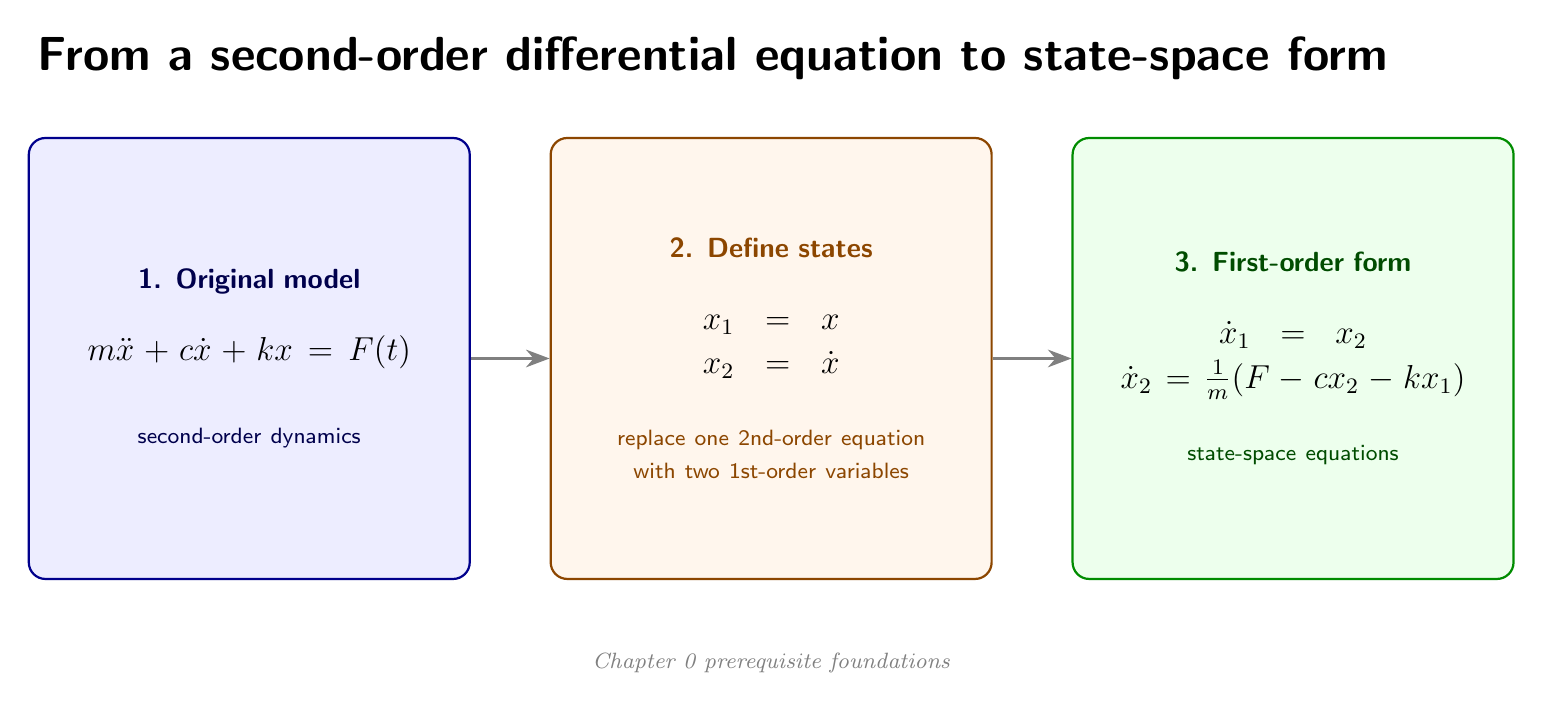
\begin{tikzpicture}[
    font=\sffamily,
    node distance=10mm and 10mm,
    card/.style={rectangle, rounded corners=6pt, draw=#1!55!black, thick,
        fill=#1!7, minimum width=5.6cm, minimum height=5.6cm,
        text width=5.0cm, align=center, inner sep=8pt},
]

\node[font=\sffamily\bfseries\LARGE, anchor=north west] (title) at (0,0)
    {From a second-order differential equation to state-space form};

\node[card=blue, below=of title.west, anchor=north west] (m1)
    {\textcolor{blue!30!black}{\bfseries 1. Original model}\\[14pt]
     {\large $m\ddot{x} + c\dot{x} + kx = F(t)$}\\[18pt]
     \textcolor{blue!30!black}{\footnotesize second-order dynamics}};

\node[card=orange, right=of m1] (m2)
    {\textcolor{orange!55!black}{\bfseries 2. Define states}\\[14pt]
     {\large $x_1 = x$}\\[4pt]
     {\large $x_2 = \dot{x}$}\\[14pt]
     \textcolor{orange!55!black}{\footnotesize replace one 2nd-order equation with two 1st-order variables}};

\node[card=green, right=of m2] (m3)
    {\textcolor{green!30!black}{\bfseries 3. First-order form}\\[14pt]
     {\large $\dot{x}_1 = x_2$}\\[4pt]
     {\large $\dot{x}_2 = \tfrac{1}{m}(F - c x_2 - k x_1)$}\\[14pt]
     \textcolor{green!30!black}{\footnotesize state-space equations}};

\draw[-{Stealth[length=3mm]}, thick, gray] (m1.east) -- (m2.west);
\draw[-{Stealth[length=3mm]}, thick, gray] (m2.east) -- (m3.west);

\node[below=8mm of m2.south, text=gray, font=\itshape\footnotesize]
    {Chapter 0 prerequisite foundations};

\end{tikzpicture}
\end{document}
